\chapter{THIẾT KẾ GIẢI THUẬT ĐIỀU KHIỂN}
     \section{Lưu đồ giải thuật chung cho robot}
          \begin{figure}[H]
               \centering
               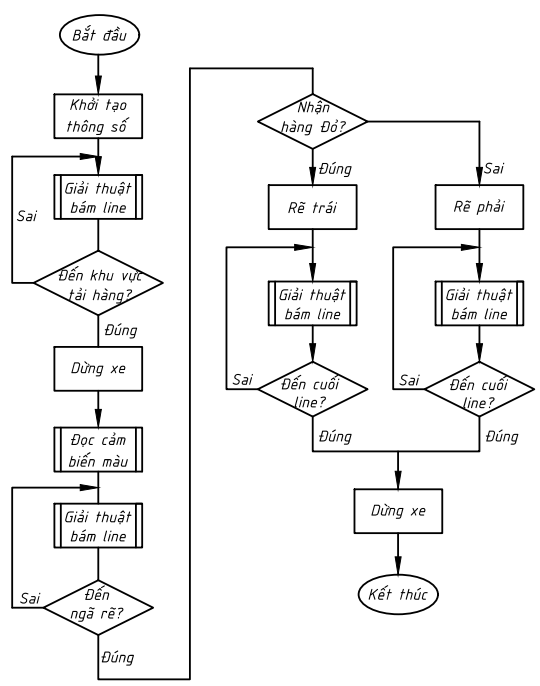
\includegraphics[width=0.7\textwidth]{pictures/chapter7/flow1.png}
               \caption{Lưu đồ giải thuật chung}
               \label{flow1}
          \end{figure}
     \section{Thiết lập sa bàn}
          \hspace*{0.6cm}Hình ảnh sa bàn đầu bài
          \begin{figure}[H]
               \centering
               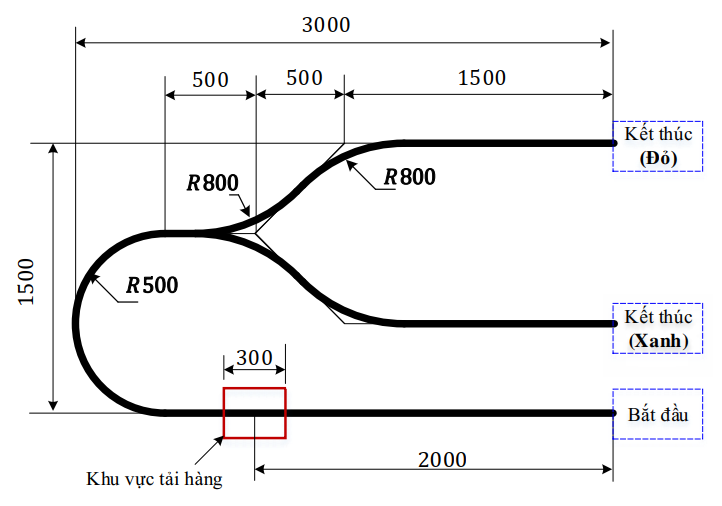
\includegraphics[width=0.7\textwidth]{pictures/chapter7/saban.png}
               \caption{Sa bàn}
               \label{race}
          \end{figure}
          \hspace*{0.6cm}Phân đoạn sa bàn
          \begin{figure}[H]
               \centering
               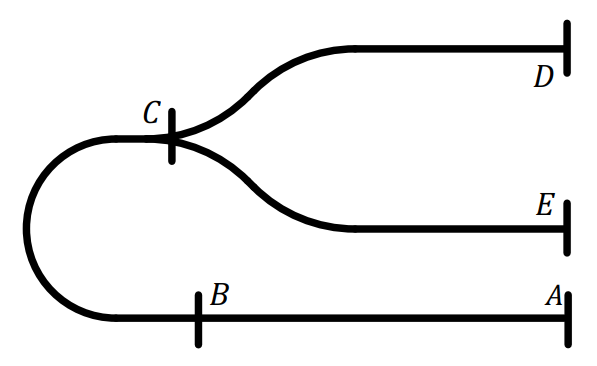
\includegraphics[width=0.6\textwidth]{pictures/chapter7/cut_saban.png}
               \caption{Phân đoạn sa bàn}
               \label{cut_race}
          \end{figure}
          \hspace*{0.6cm}Trong đó:
          \begin{itemize}
               \item $A$: điểm bắt đầu, cần đặt xe sao cho xe bắt được line đen.
               \item $B$: vị trí xe dừng để nhận hàng, được đánh dấu bằng một vạch line đen cắt
               ngang với chiều dài 50mm và chiều rộng 26mm. Với kích thước như đầu bài, vạch tải
               hàng được nhận biết khi có 3 cảm biến phát hiện được giá trị vượt ngưỡng đã đặt trước.
               \item $C$: điểm rẽ hướng, Nhận biết bằng điều kiện số cảm biến nhận line đen và phân biệt với vị trí $B$ nhờ điều kiện có tải hay không.
               \item $D$: điểm kết thúc nếu nhận hàng màu đỏ, nhận biết điểm kết thúc khi xe đi hết đường line đen.
               \item $E$: điểm kết thúc nếu nhận hàng màu xanh, nhận biết điểm kết thúc khi xe đi hết đường line đen
          \end{itemize}
     \section{Giải thuật}
          \subsection{Giải thuật bám line}
               \hspace*{0.6cm}Giá trị analog đọc về từ 5 cảm biến dò line được tính toán bằng giải thuật nội suy
               trung bình trọng số, đưa ra được sai số $e_2$ là sai số giữa tâm cảm biến và tâm đường
               line. Đưa sai số $e_2$ là đầu vào bộ điều khiển PID hệ thống để tính toán ra vận tốc
               bánh trái và vận tốc bánh phải của động cơ. Từ vận tốc hai bánh có được đưa vào bộ
               điều khiển PID của 2 động cơ để tính toán cấp xung cho 2 động cơ tương ứng.
          \subsection{Giải thuật hoàn thành đầu bài}
               \hspace*{0.6cm}Giai đoạn 1, robot đi từ điểm bắt đầu $A$ đến điểm tải hàng $B$ bằng giải thuật bám line. Khi gặp vạch tải hàng, 3 trên 5 cảm biến dò line sẽ có giá trị vượt ngưỡng (cho thấy cả 3 cảm biến đều đã nhìn thấy line đen)
               xét cùng với trạng thái của cờ \textit{empty} (thể hiện tình trạng có tải của xe), khi đó xe dừng và cờ báo xe dừng chờ nhận tải hàng được kích hoạt.\\
               \hspace*{0.6cm}Giai đoạn 2, giai đoạn tải hàng. Khi đặt gói hàng lên xe, thì cảm biến màu sẽ đọc
               tín hiệu màu của gói hàng. Khi cảm biến đã xác nhận được màu của gói hàng là Xanh hoặc
               Đỏ, xe đợi 5s sau đó tiếp tục chạy.\\
               \hspace*{0.6cm}Giai đoạn 3, robot đi từ điểm tải hàng $B$ đến điểm rẽ hướng $C$. Bằng cách đếm xung encoder, robot nhận biết được khúc vào cua bán kính $R500$ để giảm tốc độ xuống để vào line, robot sẽ đi qua đoạn cua $R500$ sau đó đi thẳng đến điểm $C$. Xe nhận biết
               được đoạn rẽ bằng số lượng cảm biến, khi 3 trên 5 cảm biến có tín hiệu và cờ báo hiệu rẽ được kích hoạt,
               xe nhận biết được sẽ rẽ sang bên đường tương ứng với màu sắc khi xác nhận tại điểm $B$.\\
               \hspace*{0.6cm}Giai đoạn 4, robot đi từ điểm rẽ hướng $C$ đến điểm kết thúc $D$ tương ứng màu Đỏ
               hoặc $E$ tương ứng màu Xanh. Bằng giải thuật bám line, xe rẽ hướng và qua 2 đoạn
               cua $R800$ sau đó đi thẳng về điểm kết thúc tương ứng.
               \begin{figure}[H]
                    \centering
                    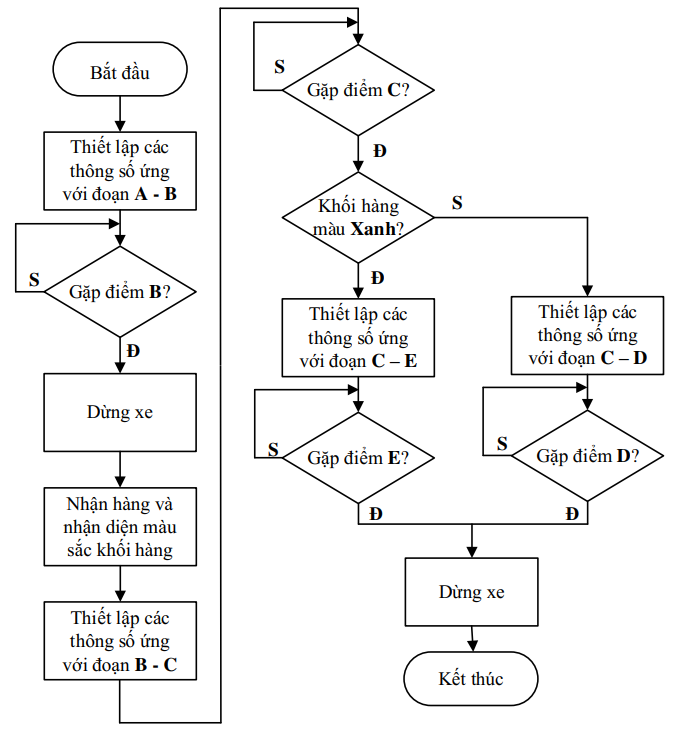
\includegraphics[width=0.8\textwidth]{pictures/chapter7/flow2.png}
                    \caption{Lưu đồ giải thuật cụ thể trên từng đoạn sa bàn}
                    \label{flow2}
               \end{figure}



